\documentclass[main.tex]{subfiles}
\begin{document}
流变学(rheology)在牛津语言网站上的释义是:研究物质的变形和流动——特别是液体的非牛顿流动和固体的塑性流动——的科学(The branch of science that deals with the deformation and flow of matter, esp. the non-Newtonian flow of liquids and the plastic flow of solids)。

流变学是一门力学,属于经典力学范畴。力学包括静力学(statics)、运动学(kinematics)和动力学(dynamics)三种问题。静力学集中考虑物体处于力的平衡之下的问题。运动学定量描述物体的位置和状态随时间的变化关系。动力学研究和分析物体运动状态改变的原因。\cite[p.~1]{邓文基2009大物上}

\begin{wrapfigure}{R}{0.25\textwidth}
\centering
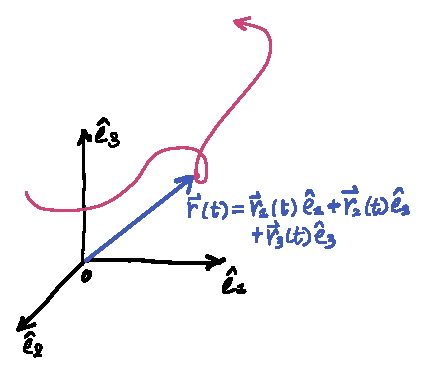
\includegraphics[width=0.25\textwidth]{images/I.1.1.eps}
\caption{质点运动学}
\label{fig:I.1.1}
\end{wrapfigure}


\end{document} 
